\documentclass{../sftex/sftex}

\usepackage{graphicx}

\title{Representação de máquinas de Turing usando \emph{JFlap}}
\author{Antonio Luiz Rosa Teixeira, Gustavo Zambonin}
\email{\{antonio.teixeira,gustavo.zambonin\}@grad.ufsc.br}
\src{https://github.com/zambonin/ufsc-ine5415}
\uniclass{Teoria da Computação}
\classcode{UFSC-INE5415}

\begin{document}

\maketitle

\section*{Questão 1}

\begin{itemize}

    \item \textbf{Descrição da linguagem}: $L(M) = \{0^{2^{n}}, \; n \geq 0\}$

    \item \textbf{Descrição do funcionamento}: A máquina, primeiramente,
        marca um símbolo vazio no começo da fita para que saiba o seu início.
        Depois, conta os zeros aos pares, marcando-os e voltando ao início da
        fita. Se ainda existirem zeros desmarcados, o processo se repetirá,
        mas apenas marcando um a cada quatro zeros, e assim por diante,
        respeitando as potências de 2. O processamento da máquina força o
        estado de rejeição na primeira marcação dos zeros se não encontrar uma
        entrada de tamanho $2^{n}$.

    \item \textbf{Codificação da máquina}:

        \begin{figure}[htbp]
            \centering
            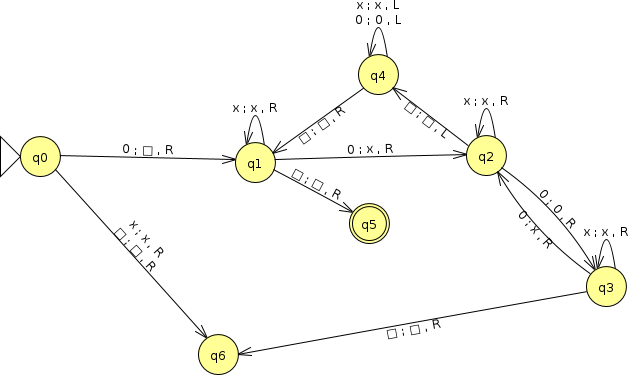
\includegraphics[scale=0.5]{images/questao1_ss.png}
        \end{figure}

    \item \textbf{Testes realizados}:

        \begin{figure}[htbp]
            \centering
            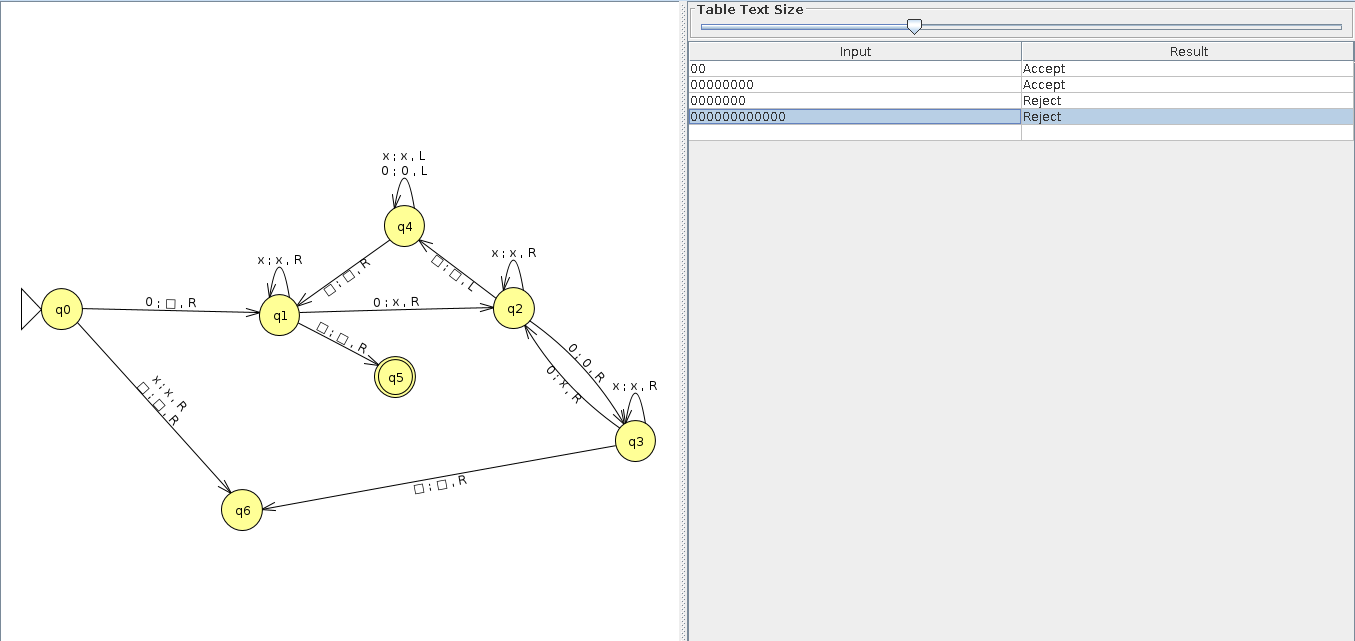
\includegraphics[width=\textwidth]{images/questao1_inputs.png}
        \end{figure}

\end{itemize}

\section*{Questão 2}

\begin{itemize}

    \item \textbf{Descrição da linguagem}:
        $L(M) = \{a^{i}b^{j}c^{k} \mid i \times j = k \land i,j,k \geq 1\}$

    \item \textbf{Descrição do funcionamento}: A máquina marca um A e a
        quantidade inteira de letras B, e a mesma quantidade de letras C,
        fazendo uma operação similar à soma de multiplicações triviais. Ao
        final da marcação de letras C, as letras B são desmarcadas e a próxima
        letra A é marcada, e assim por diante. Se a multiplicação não
        apresentar seu resultado correto, lembrando que todas as letras
        precisam aparecer pelo menos uma vez, a máquina rejeitará a entrada.

    \item \textbf{Codificação da máquina}:

        \begin{figure}[htbp]
            \centering
            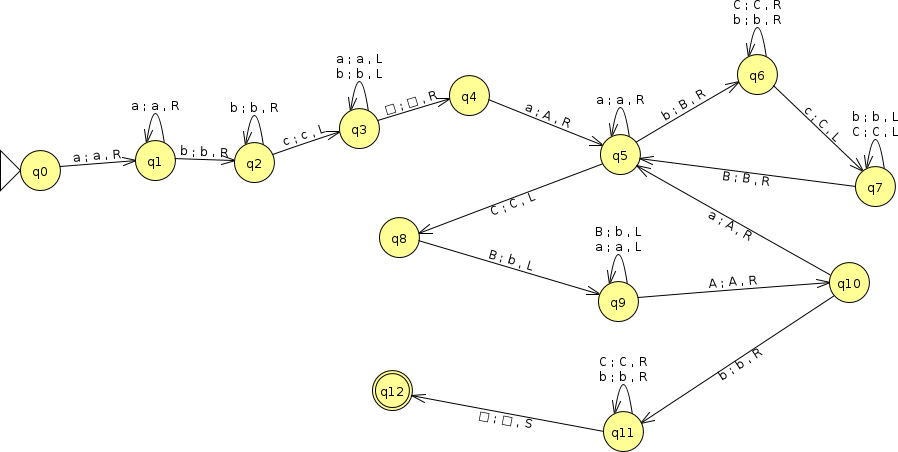
\includegraphics[scale=0.5]{images/questao2_ss.png}
        \end{figure}

	\item \textbf{Testes realizados}:

        \begin{figure}[htbp]
            \centering
            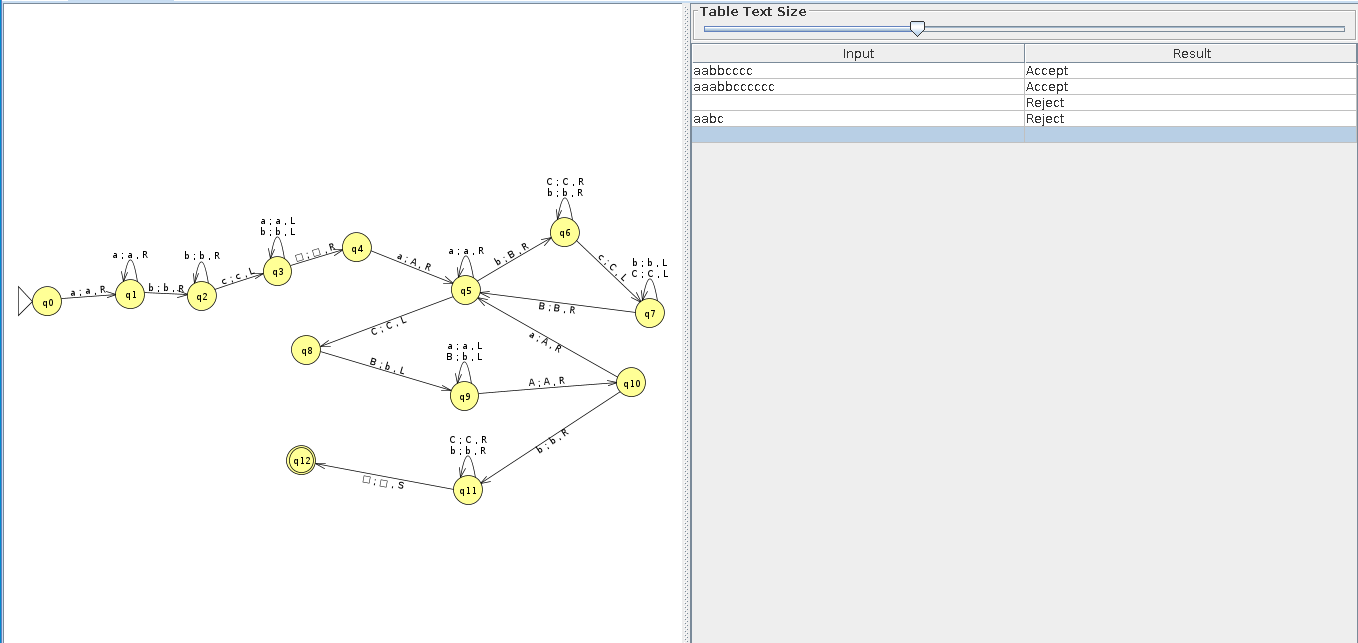
\includegraphics[width=\textwidth]{images/questao2_inputs.png}
        \end{figure}

\end{itemize}

\section*{Questão 3}

\begin{itemize}

    \item \textbf{Descrição da linguagem}:
        $L(M) = \{ \#x_1\#x_2 \cdots \#x_n \mid x_i \in \Sigma = {\{0,1\}}^*
            \land x_i \neq x_j \; \forall \; i \neq j\}$

    \item \textbf{Descrição do funcionamento}: A máquina compara
        $x_i$ e $x_j$, $\forall i\neq j$, exceto pela palavra vazia, garantida
        no início do procedimento. Após esta garantia, um $x_i$ é fixado e
        comparado com $x_{i+1}, x_{i+2}, \ldots, x_n$. Depois do final dessa
        comparação, a próxima subpalavra, $x_{i+1}$, é fixada e comparada com
        os elementos posteriores, separados pelo \#, até que este não seja
        mais encontrado na entrada, significando o fim da mesma.

    \item \textbf{Codificação da máquina}:

        \begin{figure}[htbp]
            \centering
            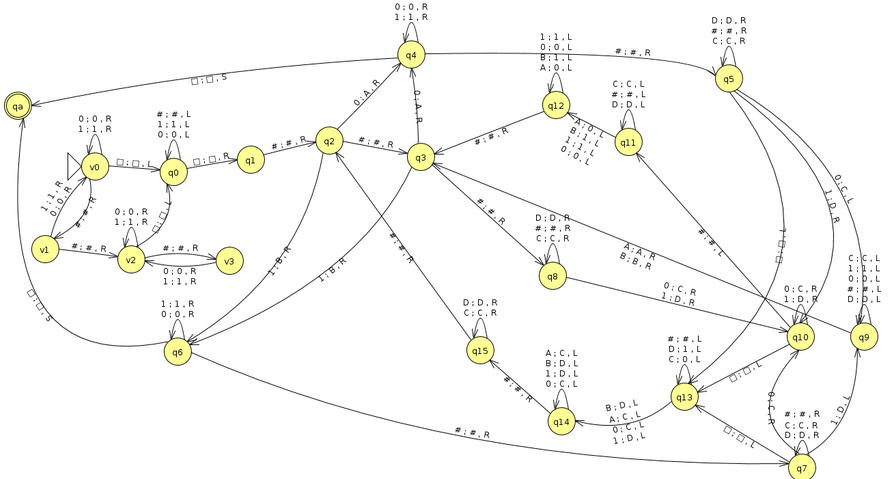
\includegraphics[scale=0.5]{images/questao3_ss.png}
        \end{figure}

    \item \textbf{Testes realizados}:

        \begin{figure}[htbp]
            \centering
            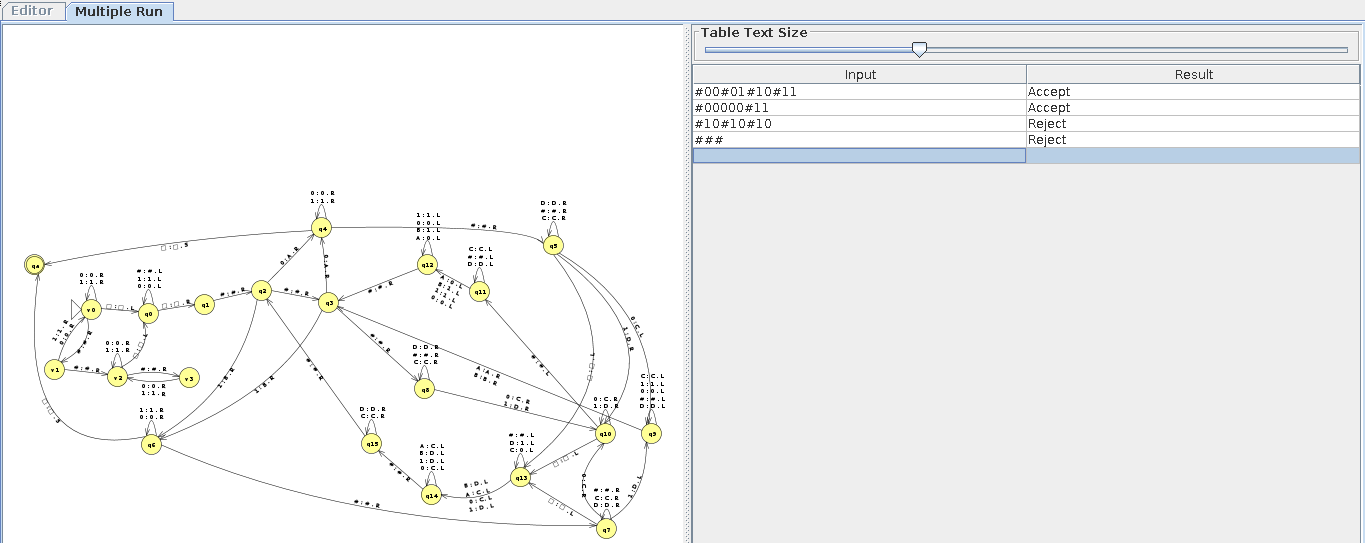
\includegraphics[width=\textwidth]{images/questao3_inputs.png}
        \end{figure}

\end{itemize}

\end{document}
